\documentclass[11pt]{article}
% ---------------------------------------------------------------------------
% Overleaf-ready. Compile with pdfLaTeX + BibTeX. Tables in tables/ and figures in
% figures/ are generated by scripts/run_all.py; do not edit them by hand.
% ---------------------------------------------------------------------------
\usepackage[a4paper,margin=2.5cm]{geometry}
\usepackage[T1]{fontenc}
\usepackage{mathptmx}
\usepackage[scaled=0.92]{helvet}
\usepackage{microtype}
\usepackage{amsmath,amssymb}
\usepackage{booktabs}
\usepackage{graphicx}
\usepackage{caption}
\usepackage{threeparttable}
\usepackage{courier}
\usepackage[section]{placeins}
\usepackage{setspace}
\usepackage{xcolor}
\usepackage[numbers,sort&compress]{natbib}
\usepackage[colorlinks=true,linkcolor=blue!50!black,citecolor=blue!50!black,urlcolor=blue!50!black]{hyperref}
\usepackage{url}
\graphicspath{{figures/}}
\captionsetup{font=small,labelfont=bf}
\setstretch{1.15}
\newcommand{\pct}[1]{#1\%}
\newsavebox{\fitbox}
\newcommand{\fittable}[1]{\sbox{\fitbox}{\input{tables/#1}}\ifdim\wd\fitbox>\linewidth\resizebox{\linewidth}{!}{\usebox{\fitbox}}\else\usebox{\fitbox}\fi}

\title{Expiry Moves the Close, Not the Day:\\Natural Experiments from India's Changing Options Expiry Calendar}
% TODO (author): check name, affiliation and e-mail before submitting.
\author{Vikash\thanks{Department of Computer Science and Engineering (AI \& ML), Chandigarh University, India. E-mail: \texttt{vikashyadav123411@gmail.com}. Code and replication files: \url{https://github.com/vicky123411/india-options-expiry-effects}.}}
\date{October 2026}

\begin{document}
\maketitle

\begin{abstract}
\noindent
Index options in India are the most heavily traded derivatives in the world, and a large share of the trading now happens on the day a contract expires. Regulators and commentators often argue that expiry days destabilise the market. I test this using a feature of the Indian market that works as a series of natural experiments: between 2016 and 2025 the exchanges changed the expiry weekday of options on the indices studied here eleven times. If expiry causes volatility, the volatile day should move when the expiry day moves.

Using daily data for four indices (2014--2026) and one-minute data for three of them (2021--2026), I find that expiry makes the trading day as a whole at most slightly more volatile. The pooled estimate for weekly expiries is $-2.4\%$ in variance, with a 95\% interval of $-8\%$ to $+4\%$. What expiry does change is the end of the day. In the 15:00--15:30 window, whose average price set the settlement value until August 2026, variance is 53\% higher on weekly expiry days and 67\% higher on monthly ones. When an expiry moves to a new weekday, this volatile last half hour moves with it. In all five changes covered by the minute data that gave a weekday a new expiry, that weekday's closing window became more volatile, and it became calmer in four of the five changes that took an expiry away; the exception is a weekday that received another index's expiry on the same day. None of 1,000 placebo calendars produces a closing-window effect as large as the real calendar's.

The settlement-window effect remained large after SEBI's November 2024 measures and was largest after its July 2025 interim order against alleged expiry-day manipulation. There is little evidence of pinning to strikes. Adding the expiry calendar does not improve daily volatility forecasts. If the concern is market stability, the results point to how settlement prices are set, rather than how often contracts expire, as the place to act; an early look at the closing auction introduced in August 2026 shows no reduction yet.

\medskip
\noindent\textbf{Keywords:} options expiry; settlement price; intraday volatility; natural experiment; weekly options; 0DTE; India; market microstructure.\\
\noindent\textbf{JEL:} G13, G14, G18.
\end{abstract}

% ===========================================================================
\section{Introduction}
India's index options market grew into the largest derivatives market in the world in less than a decade. Most of that growth came from short-dated contracts. In 2024, 59\% of all Nifty~50 option contracts traded during the year were traded on the very day they expired, compared with 9--11\% in 2014--2018 (Figure~\ref{fig:activity}). Most of this trading is by individuals, and SEBI's studies find that about nine in ten individual traders lose money \citep{sebi2024study,sebi2025study}.

Regulators have responded by restricting the product. In October 2024 SEBI limited each exchange to one weekly expiry and raised margins on expiry days \citep{sebi2024circular}. In July 2025 it issued an interim order alleging that a large trading firm manipulated index levels on expiry days \citep{sebi2025janestreet}. Behind these steps is a widely held but rarely tested belief: that expiry days make the underlying market unstable.

Whether they do is an empirical question. Theory points both ways:
\begin{itemize}
\item \textbf{Expiry could add volatility.} Option writers who delta-hedge short positions trade with the market as gamma rises near expiry \citep{ni2021,baltussen2021,barbon2020}. Traders with large positions may also try to move the settlement price \citep{kumar1992,hillion2004,comertonforde2011}.
\item \textbf{Expiry could reduce volatility.} Hedgers who are long gamma trade against price moves, which can pin prices to strikes \citep{avellaneda2003,ni2005,golez2012}.
\end{itemize}
The evidence from the US ``zero-days-to-expiry'' (0DTE) boom is mixed \citep{dim2024,brogaard2023}. Evidence from India mostly compares expiry days with other days \citep{vipul2005,agarwalla2013,chhimwal2025}. That comparison is hard to read, because expiry days fall on fixed weekdays and weekdays differ for many other reasons.

\paragraph{This paper's design.} India's expiry calendar was rearranged over and over:
\begin{itemize}
\item Bank Nifty gained weekly Thursday options in 2016 and Nifty in 2019.
\item Bank Nifty moved to Wednesday in 2023.
\item Sensex options were relaunched with Friday expiry in 2023, moved to Tuesday in 2025, and to Thursday later in 2025.
\item Nifty moved to Tuesday in September 2025, on the same day that Sensex moved to Thursday.
\item Weekly contracts on Bank Nifty and on smaller indices were abolished in November 2024.
\end{itemize}
Each change moves the expiry from one weekday to another for one index while the others stay put. Holidays add more variation, because an expiry that falls on a holiday moves to the previous trading day.

I build the full calendar of six index option products from 2014 to 2026 from the exchanges' rules. It matches, with zero mismatches, all 932 Nifty and Bank Nifty expiry days visible in NSE's contract files and all 148 Sensex expiry dates in an independent option dataset. I then ask a sharp question: \emph{when the expiry day moves, does the volatility move with it?}

\paragraph{Findings.}
\begin{enumerate}
\item \textbf{The day as a whole is at most slightly more volatile.} Comparing each index with itself in the same week and against its normal weekday pattern, weekly expiry days have $-2.4\%$ variance (95\% interval $-8.4\%$ to $+4.0\%$) and monthly expiry days $+5.7\%$ ($-4.0\%$ to $+16.3\%$). Placebo calendars confirm that these estimates are typical of random weekdays. Event-window estimates around the calendar changes are somewhat higher (about $+15\%$ for a weekday gaining an expiry), so modest whole-day effects cannot be excluded.
\item \textbf{The settlement window is much more volatile.} Until August 2026, the official closing value of an index, and therefore the settlement price of expiring options, was an average of prices from 15:00 to 15:30. In that half hour, variance is 53\% higher on weekly expiry days and 67\% higher on monthly ones. The effect is largest for Sensex (about $+150\%$) and spills over to indices whose own options are not expiring.
\item \textbf{The effect follows the calendar.} In all five changes covered by minute data that gave a weekday a new expiry, that weekday's closing window became more volatile (four of the five individually significant), and in four of the five changes that took an expiry away it became calmer, three of them significantly (Figure~\ref{fig:moving}). The exception, Nifty's Thursday in September 2025, received Sensex's expiry on the same day. Stacking the six changes, the new weekday's closing-window variance rises by 65\% and the old weekday's falls by 31\%. In the pooled regressions, none of 1,000 placebo calendars produces a closing-window estimate as large as the real one.
\item \textbf{Regulation has not removed it.} The effect remained large and significant after SEBI's November 2024 measures, although point estimates were somewhat lower in the months that followed, and it was largest after the July 2025 interim order. There is little evidence of pinning to strikes.
\item \textbf{For Bank Nifty in 2023--2025}, the period covered by SEBI's allegations, the last half hour tended to reverse the rest of the day's move on expiry days but not on other days. This test was chosen to match the allegations and is suggestive only.
\end{enumerate}

\paragraph{Contributions.}
\begin{itemize}
\item I use \emph{all} of India's expiry-calendar changes as natural experiments, rather than a single change \citep{chhimwal2025} or a comparison of expiry days with other days \citep{vipul2005,agarwalla2013}. The 2024--2025 changes, including the September 2025 Nifty--Sensex swap, have not been studied before.
\item I locate the effect precisely: the settlement window, not the trading day. This reconciles the popular view (``expiry days are wild'') with the near-zero daily estimates. For most investors the day is not riskier; the price used for settlement is.
\item The results speak to policy. SEBI's 2024 measures were motivated mainly by investor protection, but to the extent that market stability is the concern, the volatility that expiry causes sits in how the settlement price is formed, not in the trading day as a whole. That is the target of the closing auction NSE introduced on 3 August 2026 \citep{nse2026casgolive}; whether it works is not yet clear.
\item The paper complements earlier work on Nifty volatility forecasting. Knowing the expiry calendar does not improve next-day forecasts, which is consistent with the effect being confined to the last half hour.
\end{itemize}

% ===========================================================================
\section{Institutional background}\label{sec:background}
\paragraph{Products.}
\begin{itemize}
\item The NSE lists options on the Nifty~50, Nifty Bank (``Bank Nifty''), Nifty Financial Services and Nifty Midcap Select indices.
\item BSE lists options on the Sensex and Bankex.
\item All are cash-settled European options. At expiry they settle against the official closing value of the index on the expiry day.
\item Until 3 August 2026, each constituent stock's closing price was the volume-weighted average price of its trades between 15:00 and 15:30, and the index's closing value was computed from these. The closing auction session that started on 3 August 2026 replaced this rule for F\&O stocks \citep{nse2026cassop,nse2026casgolive}. My main sample therefore ends on 31 July 2026.
\end{itemize}

\paragraph{The expiry calendar.}
\begin{itemize}
\item Table~\ref{tab:rules} lists every rule. Weekly contracts expire every week on a fixed weekday, and the monthly contract expires on the last such weekday of the month.
\item In the week of a monthly expiry, no separate weekly contract is listed. This matters only when the two weekdays differ (Bank Nifty, September 2023 -- February 2024).
\item If the scheduled day is a holiday, contracts expire on the previous trading day.
\item The changes came from several sources: competition between the exchanges, a wish to avoid expiries clustering on one day, SEBI's measures of October 2024 (implemented from 20 November 2024) \citep{sebi2024circular}, and a SEBI-directed move of all NSE expiries to Tuesday and BSE expiries to Thursday from 1 September 2025 \citep{nse2025expiry,bse2025expiry}.
\item None of these changes was a response to volatility on a particular weekday, although the November 2024 removal of weekly contracts was aimed at expiry-day speculation in general. That the choice of weekday is unrelated to that weekday's volatility trend is the identifying assumption discussed in Section~\ref{sec:design}.
\end{itemize}

\paragraph{Regulatory events.}
\begin{itemize}
\item \textbf{SEBI's October 2024 circular} \citep{sebi2024circular} did four things. It allowed one weekly benchmark contract per exchange. It raised minimum contract sizes. It added an extra 2\% margin on short options on expiry day. It removed calendar-spread margin benefits on expiry day.
\item \textbf{On 3 July 2025} SEBI issued an interim order against the Jane Street group \citep{sebi2025janestreet}. The order alleged that, on expiry days between 2023 and 2025, the group traded index stocks and futures in large size to move index levels. The alleged patterns were buying in the morning and selling later in the day, and ``extended marking the close'' near the settlement window, while holding larger opposite positions in options.
\item These are allegations in an interim order. I use the date only to ask whether the expiry-day patterns changed afterwards.
\end{itemize}

\begin{figure}[t]
\centering
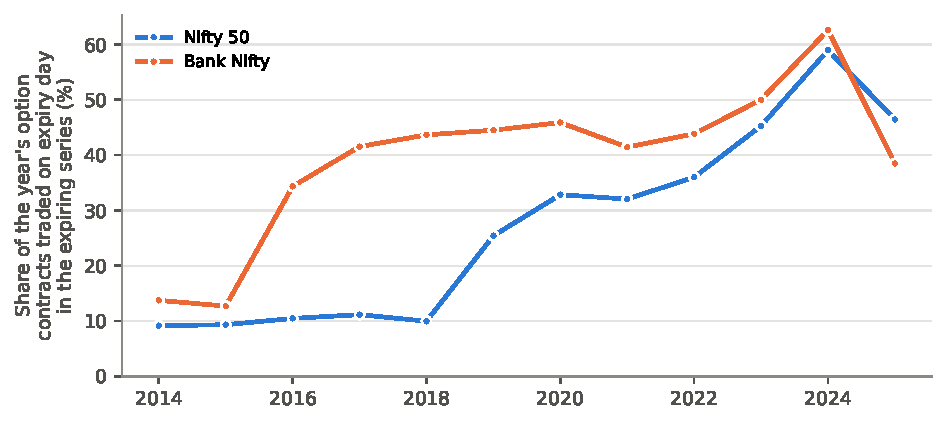
\includegraphics[width=0.72\textwidth]{fig1_activity.pdf}
\caption{\textbf{The rise of expiry-day trading.} Share of all option contracts traded in a year that were traded on an expiry day, in the series expiring that day. Source: NSE F\&O contract files.}
\label{fig:activity}
\end{figure}

% ===========================================================================
\section{Data and measurement}\label{sec:data}
\paragraph{Daily prices.}
\begin{itemize}
\item \textbf{Indices:} daily open, high, low and close for the Nifty~50, Nifty Bank, S\&P BSE Sensex and Nifty Midcap~50 from Yahoo Finance, January 2014 to July 2026.
\item \textbf{Why Midcap~50:} it is the index least exposed to large-cap index options. Its ``own'' options are Nifty Midcap Select options, a small market built from similar stocks.
\item \textbf{Cleaning:} I drop weekend special sessions, Diwali \emph{Muhurat} evening sessions and incomplete bars. The holiday calendar is rebuilt from the days on which neither NSE's contract files nor the price data show trading. It matches the exchanges' published holiday lists for 2024--2025.
\item \textbf{Sample:} 12,312 index-days (Table~\ref{tab:sample}).
\end{itemize}

\paragraph{One-minute prices.}
\begin{itemize}
\item One-minute index bars come from a public dataset (CC~BY-NC~4.0) for Nifty~50 and Bank Nifty (May 2021 -- 2 July 2026) and Sensex (September 2022 -- 2 July 2026). That is 3,428 index-days with full sessions.
\item Daily ranges rebuilt from the minute bars correlate 0.996--0.999 with the daily data.
\end{itemize}

\paragraph{Option contract files.}
\begin{itemize}
\item NSE's end-of-day F\&O files (``bhavcopy'') for Nifty and Bank Nifty options, 2014 -- June 2026, give contracts traded and open interest by strike and expiry.
\item I use them to verify the expiry calendar, to measure expiry-day trading (Figure~\ref{fig:activity}), and for the pinning tests.
\item \textbf{Calendar check:} a day is an observed expiry day if a series traded on its own expiry date. When the exchange's label is a holiday, the observed expiry day is the series' last trading day. The rule-based calendar agrees on all 444 Nifty and 488 Bank Nifty expiry days. The only rule-based expiry days absent from the files are two days in a gap in the files (November 2020).
\item For Sensex, all 148 expiry dates of an independent one-minute option dataset (August 2023 -- July 2026) are expiry days in the calendar. Eight calendar expiry days are absent from that dataset: six at its end (May--July 2026), where its coverage thins, and two in the middle (31 October 2024, a Diwali-related holiday shift, and 30 October 2025), which could not be checked.
\end{itemize}

\paragraph{Volatility measures.} All variances are in $\%^2$, and outcomes are their logs. A coefficient $b$ therefore means the variance is $100(e^{b}-1)\%$ higher.
\begin{itemize}
\item \textbf{Whole session, daily data:} the Garman--Klass variance \citep{garman1980},
\[
\sigma^2_{GK} = 0.5\,(\ln H-\ln L)^2-(2\ln 2-1)(\ln C-\ln O)^2.
\]
Robustness uses Parkinson's \citep{parkinson1980} and Rogers--Satchell's \citep{rogers1991} estimators, the squared open-to-close return, close-to-close variance (overnight plus session), and the squared overnight gap.
\item \textbf{Whole session, minute data:} realized variance from five-minute returns, 09:15--15:30.
\item \textbf{Settlement window:} realized variance of one-minute returns from 15:00 to 15:30.
\item \textbf{Intraday profiles:} realized variance in each 15-minute slot.
\end{itemize}

\begin{table}[t]
\centering
\caption{\textbf{The expiry calendar of Indian index options.} Each row is a rule, valid from its start date until the next row of the same product. Weekly contracts expire every week on the weekday shown; the monthly contract on the last such weekday of the month. If that day is a holiday, contracts expire on the previous trading day. NIFTY, BANKNIFTY, FINNIFTY and MIDCPNIFTY trade on NSE; SENSEX and BANKEX on BSE.}
\label{tab:rules}
\scriptsize
\fittable{rules}
\end{table}

\begin{table}[t]
\centering
\caption{\textbf{Sample.} Trading days January 2014 -- July 2026 after cleaning; number of own weekly and monthly expiry days; days on which another large index's options expire; annualized volatility (close-to-close variance, overnight plus Garman--Klass).}
\label{tab:sample}
\small
\fittable{sample}
\end{table}


% ===========================================================================
\section{Empirical design}\label{sec:design}
\paragraph{Treatment variables.} For index $i$ on day $t$:
\begin{itemize}
\item \textsc{OwnWeekly}$_{it}$ and \textsc{OwnMonthly}$_{it}$ indicate that the index's own options have a weekly or monthly expiry. The monthly expiry is also the expiry of index futures.
\item \textsc{OtherLarge}$_{it}$ indicates that options on another of Nifty, Bank Nifty and Sensex expire. These three indices share many stocks.
\item \textsc{OtherSmall}$_{it}$ indicates the expiry of Fin Nifty, Midcap Select or Bankex options.
\end{itemize}

\paragraph{Main specification.}
\begin{equation}\label{eq:main}
\begin{split}
y_{it} = {}& \beta_w\,\textsc{OwnWeekly}_{it} + \beta_m\,\textsc{OwnMonthly}_{it} + \gamma_1\,\textsc{OtherLarge}_{it} + \gamma_2\,\textsc{OtherSmall}_{it}\\
&+ \alpha_{i,\,\mathrm{weekday}(t)} + \delta_{i,\,\mathrm{week}(t)} + \varepsilon_{it}.
\end{split}
\end{equation}
\begin{itemize}
\item The index-by-weekday effects $\alpha$ remove each index's normal weekday pattern.
\item The index-by-week effects $\delta$ remove that week's overall level of volatility.
\item So the $\beta$s are identified only by days whose expiry status differs from what is usual for their weekday, that is, by the calendar changes and holiday shifts. In effect, equation~\eqref{eq:main} is a difference-in-differences with treatment switching on and off at different times for different index-weekday cells.
\item Standard errors are clustered by calendar week (about 650 clusters). This allows any correlation across indices and days within a week.
\item The fixed effects are removed by alternating projections \citep{guimaraes2010,correia2016}. Small-sample corrections follow \texttt{reghdfe}.
\end{itemize}

\paragraph{Identifying assumption.}
\begin{itemize}
\item Absent the calendar change, the volatility of the weekday gaining (or losing) an expiry would have moved in parallel with the index's other weekdays.
\item Weekday effects common to the whole market, such as a change in when US macro news arrives, are absorbed in robustness checks by weekday-by-year effects and, in the strictest version, by date fixed effects. The date-effects version compares indices with each other on the same day.
\item Because the indices share stocks, an expiry of one can move the others. The date-effects estimate therefore measures own-expiry effects \emph{relative to} spillovers, and is a lower bound on the total effect.
\end{itemize}

\paragraph{Event studies.}
\begin{itemize}
\item For each of the eight major calendar changes, I take a window of $\pm 26$ weeks, cut at any other change to the same product's rules.
\item Within the window I estimate the change in the gained and the lost weekday relative to the index's other weekdays, after versus before (with weekday and week effects).
\item A stacked version pools the changes, with event-specific fixed effects. This avoids the ``forbidden comparisons'' of two-way fixed effects with staggered timing \citep{goodmanbacon2021,dechaisemartin2020,cengiz2019}.
\end{itemize}

\paragraph{Placebo calendars.}
\begin{itemize}
\item As design-based inference \citep{young2019}, I re-estimate equation~\eqref{eq:main} under 1,000 placebo calendars.
\item Each placebo keeps the dates of every rule change but assigns the weekdays at random. Weekly and monthly contracts stay on a common weekday whenever they share one in reality.
\item The $p$-value is the share of placebo estimates at least as large in absolute value as the real one.
\end{itemize}
The analysis plan, including all robustness checks and mechanism tests, was written down before these were run. It is in the replication files, with a note on what had been looked at before it was written.

% ===========================================================================
\section{Results}\label{sec:results}
\subsection{The trading day as a whole}
\begin{itemize}
\item Table~\ref{tab:main} and Figure~\ref{fig:main}A give the estimates for the whole session.
\item \textbf{Pooled:} weekly expiry days are no more volatile than other days ($\hat\beta_w=-0.024$, s.e.\ 0.032). Monthly expiry days are slightly but insignificantly more volatile ($\hat\beta_m=0.055$, s.e.\ 0.049).
\item \textbf{What the intervals rule out:} increases above 4\% in variance on weekly expiry days and above 16\% on monthly ones.
\item \textbf{Per index:} only Nifty's weekly expiry days stand out, and they are \emph{calmer}, by about 10\% ($p=0.047$, Holm-adjusted $p=0.19$).
\item \textbf{Other measures:} results are similar with other range-based measures and with close-to-close variance (Appendix Table~\ref{tab:alt}).
\item \textbf{One exception:} measured against Midcap~50 on the same day, monthly expiry days are more volatile ($+0.18$, Table~\ref{tab:robust}). Mid-caps are calmer than usual when the large indices' options expire, so this comparison partly reflects a shift of activity toward large caps.
\end{itemize}

\begin{table}[t]
\centering
\caption{\textbf{Whole session: expiry-day effects on log Garman--Klass variance.} Equation~\eqref{eq:main}. Pooled: index$\times$weekday and index$\times$week effects; per index: weekday and week effects. Standard errors clustered by calendar week in parentheses. *, **, *** = significant at 10\%, 5\%, 1\%.}
\label{tab:main}
\small
\fittable{main_lgk}
\end{table}

\begin{figure}[t]
\centering
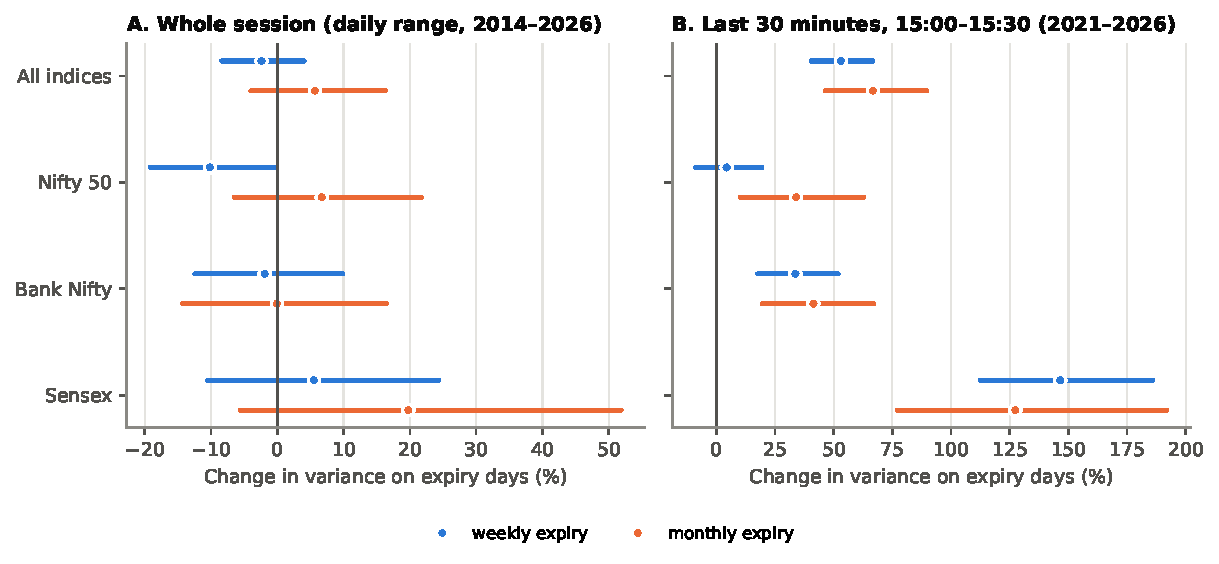
\includegraphics[width=\textwidth]{fig3_main.pdf}
\caption{\textbf{Expiry moves the close, not the day.} Estimated change in variance on own weekly (blue) and monthly (orange) expiry days with 95\% intervals. A: whole session, log Garman--Klass variance, daily data 2014--2026. B: realized variance of one-minute returns in 15:00--15:30, 2021--2026. Note the different scales.}
\label{fig:main}
\end{figure}

\begin{table}[t]
\centering
\caption{\textbf{One-minute data: whole session vs.\ settlement window.} Log realized variance of the whole session (five-minute returns) and of 15:00--15:30 (one-minute returns). Nifty 50 and Bank Nifty May 2021 -- July 2026, Sensex September 2022 -- July 2026. Fixed effects and standard errors as in Table~\ref{tab:main}.}
\label{tab:minute}
\scriptsize
\setlength{\tabcolsep}{4pt}
\fittable{minute_main}
\end{table}


\subsection{The settlement window}
\begin{itemize}
\item The minute data show where expiry does matter (Table~\ref{tab:minute}, Figure~\ref{fig:main}B).
\item \textbf{Whole session (five-minute realized variance):} again no significant effect for weekly expiries ($0.019$, s.e.\ 0.036); for monthly expiries $0.095$ (s.e.\ 0.058).
\item \textbf{15:00--15:30 window:} variance is 53\% higher on weekly expiry days ($\hat\beta_w=0.425$, s.e.\ 0.043) and 67\% higher on monthly ones ($0.511$, s.e.\ 0.066).
\item \textbf{By index:} the effect is largest for Sensex ($+146\%$ weekly, $+127\%$ monthly) and clear for Bank Nifty ($+34\%$ and $+41\%$). For Nifty it appears only for monthly expiries in the pooled 2021--2026 sample; Section~\ref{sec:policy} shows that a Nifty effect emerged after 2024.
\item \textbf{Spillovers:} expiries of another large index raise the closing-window variance by 14\%.
\end{itemize}

\subsection{Natural experiments: the effect moves with the calendar}
\begin{itemize}
\item Figure~\ref{fig:moving} shows the six calendar changes covered by the minute data. Each panel is the closing-window variance of each weekday relative to the rest of its week, in the six months before and after the change.
\item In each change that added an expiry weekday, the spike appears on the new weekday. Sensex shows it three times: Friday on relaunch, Friday $\rightarrow$ Tuesday in January 2025, and Tuesday $\rightarrow$ Thursday in September 2025. Appendix Figure~\ref{fig:movingday} shows that the whole-session profile does not follow the calendar in the same way.
\item When Nifty moved from Thursday to Tuesday, Tuesday's closing window became volatile, while Thursday's stayed high. On the same day Sensex moved \emph{into} Thursday, so Thursday kept an expiry and only changed which index expired.
\item When Bank Nifty's weekly contracts were abolished in November 2024, Wednesday's closing-window volatility disappeared.
\end{itemize}

Table~\ref{tab:events} reports the event-by-event estimates.
\begin{itemize}
\item \textbf{Stacked estimate:} gaining an expiry raises the weekday's closing-window variance by 65\% ($0.503$, s.e.\ 0.087). Losing one lowers it by 31\% ($-0.375$, s.e.\ 0.102).
\item \textbf{Timing:} the event-time profile (Figure~\ref{fig:eventtime}) is flat before the change and jumps immediately after it, with no sign of anticipation.
\item \textbf{Whole session:} gaining an expiry raises five-minute realized variance by a modest 15\% ($p=0.04$), and losing one has no detectable effect. In the daily data over all eight major changes the estimates are $+0.145$ ($p=0.07$) and $-0.016$. Any whole-day effect is therefore small compared with the closing-window effect.
\item \textbf{Caveats:} the September 2025 Nifty and Sensex changes mirror each other, so each one's ``old'' weekday received the other's expiry; and Bank Nifty's ``old'' Thursday kept its monthly expiry until February 2024. Both work against finding a fall on the old weekday.
\end{itemize}

\begin{figure}[tp]
\centering
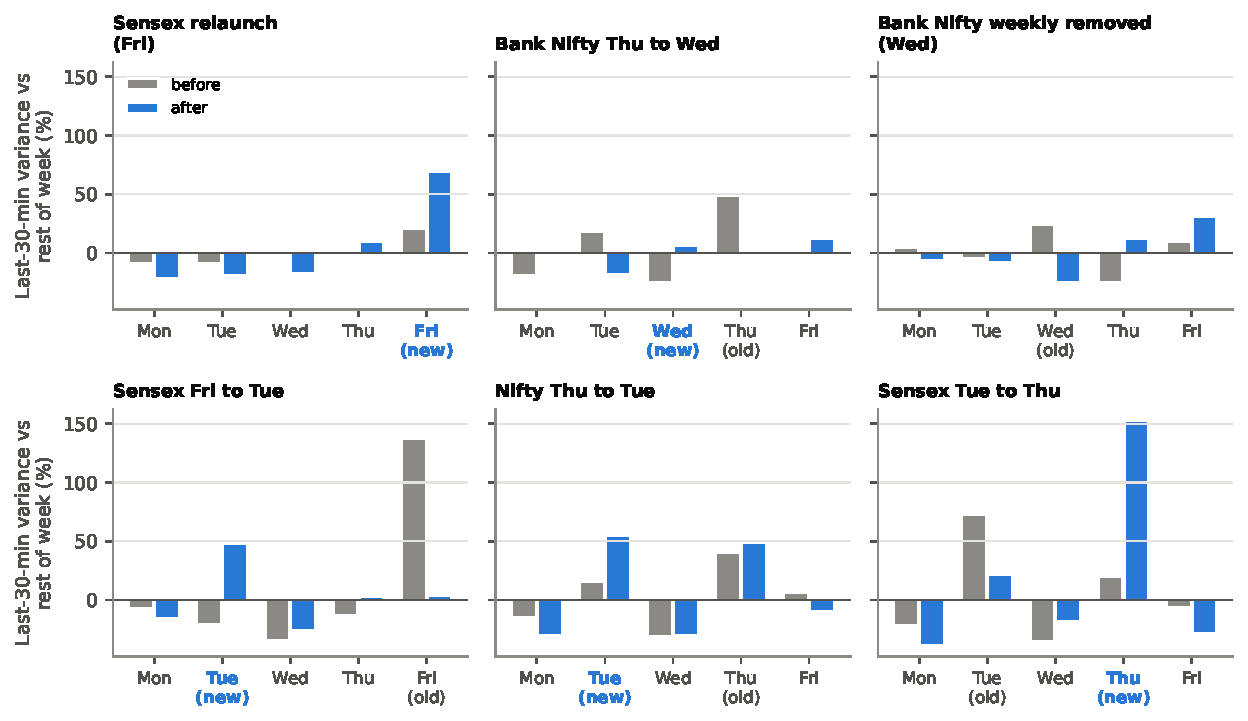
\includegraphics[width=\textwidth]{fig2_moving_close.pdf}
\caption{\textbf{The volatile closing half hour follows the expiry day.} For each calendar change with one-minute data: realized variance in 15:00--15:30 on each weekday relative to the rest of its week, in the 26 weeks before (grey) and after (blue) the change (windows cut at other changes of the same product). The new expiry weekday is in blue. In the Nifty Thursday $\rightarrow$ Tuesday panel, Thursday stays volatile because Sensex moved its expiry to Thursday on the same day.}
\label{fig:moving}
\end{figure}

\begin{table}[t]
\centering
\caption{\textbf{Natural experiments, change by change.} Difference-in-differences within a $\pm$26-week window: change in log variance of the weekday that gained (lost) the index's expiry, relative to the index's other weekdays, after vs.\ before, with weekday and week effects. Whole session: log Garman--Klass variance (last row: five-minute realized variance, 2021--2026). Last 30 minutes: one-minute realized variance 15:00--15:30 (available from 2021; Sensex from 2022). Stacked rows pool the changes with event-specific effects. $^\dagger$Midcap Select (small market). Standard errors clustered by week.}
\label{tab:events}
\scriptsize
\setlength{\tabcolsep}{3.5pt}
\fittable{events}
\end{table}

\begin{figure}[t]
\centering
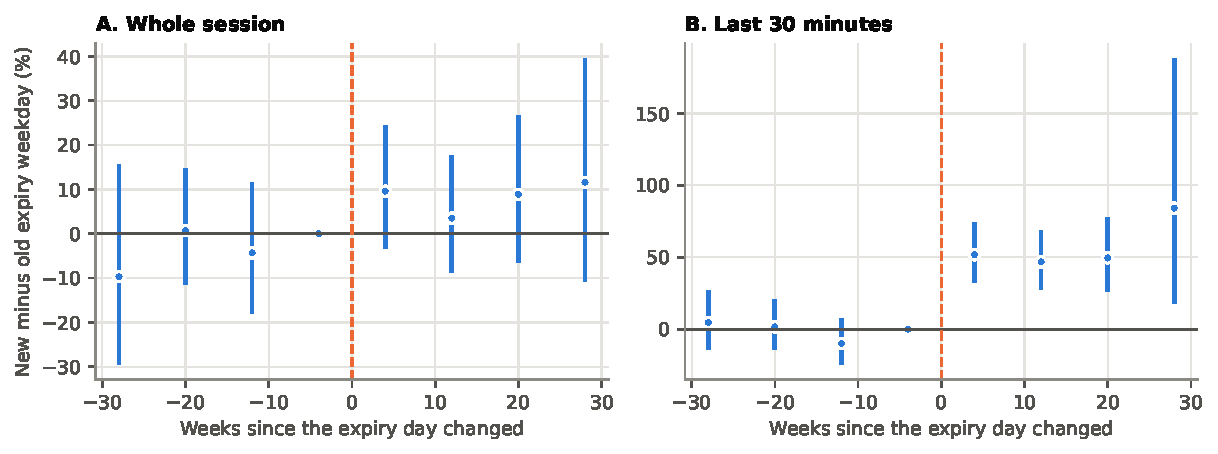
\includegraphics[width=0.95\textwidth]{fig5_event_time.pdf}
\caption{\textbf{Event time.} Stacked over the six changes with one-minute data: difference between the new and the old expiry weekday in eight-week bins around the change (the bin just before is the reference), with 95\% intervals. A: whole session (five-minute realized variance). B: 15:00--15:30.}
\label{fig:eventtime}
\end{figure}


\subsection{Robustness}
Table~\ref{tab:robust} collects the robustness checks.
\begin{itemize}
\item \textbf{Specification checks:} the settlement-window estimates barely move with weekday-by-year effects, Driscoll--Kraay standard errors \citep{driscoll1998}, holiday controls, or leads and lags of expiry.
\item \textbf{Date fixed effects:} the estimates fall to about 0.25 but remain highly significant. This comparison nets out spillovers to the other indices.
\item \textbf{Window length:} the effect is present in both 15-minute halves of the window, and already in the preceding quarter-hour, as positions are adjusted ahead of settlement.
\item \textbf{Placebo calendars:} for the pooled regression~\eqref{eq:main}, none of the 1,000 placebos gives a closing-window estimate as large as the real one ($p=0.001$, Figure~\ref{fig:placebo}). For the whole session the real estimates are ordinary ($p=0.48$ weekly, $0.22$ monthly).
\item \textbf{Holiday-shifted expiries:} using only expiries moved by a holiday, and controlling for the pre-holiday session they always fall on, the whole-session effect is $-0.07$ (s.e.\ 0.10).
\end{itemize}

\begin{table}[t]
\centering
\caption{\textbf{Robustness.} Own weekly and monthly expiry coefficients under alternative specifications. Whole session: daily data 2014--2026, log Garman--Klass variance. Last 30 minutes: one-minute data 2021--2026. ``Date effects'' compares indices on the same day (own expiry relative to the spillover on other indices). The last row gives randomization $p$-values from 1,000 placebo calendars (real rule dates, random weekdays).}
\label{tab:robust}
\scriptsize
\setlength{\tabcolsep}{4pt}
\fittable{robustness}
\end{table}


% ===========================================================================
\section{Mechanisms}\label{sec:mech}
\paragraph{Timing.} Figure~\ref{fig:intraday} estimates equation~\eqref{eq:main} separately for each 15-minute slot.
\begin{itemize}
\item The expiry effect is near zero at the open.
\item It is modest during the day (10--20\% in a typical slot) and builds through the afternoon.
\item It peaks at $+57\%$ in 15:00--15:15, the first half of the settlement window.
\item Expiries of another large index matter mainly in the first half of the settlement window (15:00--15:15).
\end{itemize}
This profile matches hedging and position management aimed at the settlement price. It does not match an information-driven or market-wide shock.

\begin{figure}[t]
\centering
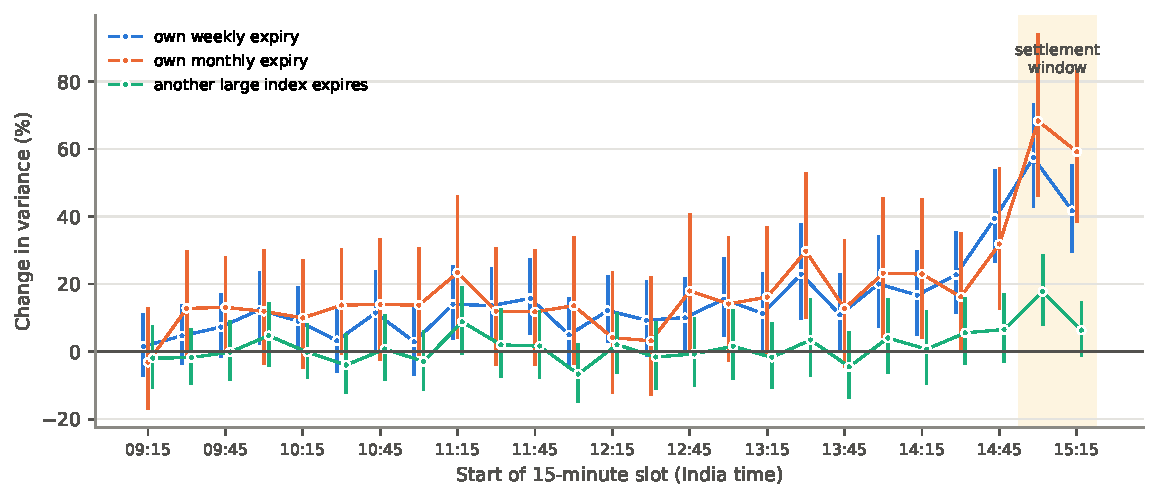
\includegraphics[width=\textwidth]{fig4_intraday.pdf}
\caption{\textbf{When in the day expiry matters.} Equation~\eqref{eq:main} estimated separately for the log realized variance of each 15-minute slot (one-minute data, 2021--2026, three indices pooled), with 95\% intervals. Shaded: the 15:00--15:30 window whose average price set the settlement value.}
\label{fig:intraday}
\end{figure}

\begin{table}[t]
\centering
\caption{\textbf{Pinning.} Top: share of official closes within 10\% of a strike step of a multiple of the step (about 0.20 with no pinning), on own expiry days and other days, and linear-probability coefficients with weekday and week effects. Bottom (Nifty and Bank Nifty, option data 2014 -- June 2026): change during the day in the distance (\% of index level) to the strike with the largest open interest at the previous close, in the nearest-expiry series; negative = moved toward the strike. The difference controls for the distance at the open, with weekday and year effects.}
\label{tab:pinning}
\scriptsize
\fittable{pinning}
\end{table}


\paragraph{Pinning.} Pinning would show up in two ways, and I test both (Table~\ref{tab:pinning}).
\begin{itemize}
\item \textbf{Closes near strikes:} official closes within 10\% of a strike step of a strike are only slightly more common on expiry days. The difference is significant only for Bank Nifty's 100-point grid (22.8\% versus 19.9\%).
\item \textbf{Moves toward the most-held strike:} on expiry days the index does not move toward the strike with the largest open interest at the previous close. If anything it moves away: by 0.11 percentage points of the index level more than on other days for Nifty ($p=0.04$), and insignificantly for Bank Nifty.
\end{itemize}
So unlike US single stocks \citep{ni2005}, India's indices are not systematically pinned. This fits a market where most option buyers are individuals who do not hedge.

\paragraph{Reversals.} SEBI's interim order described buying early on expiry days and selling into the close \citep{sebi2025janestreet}. I regress the last half-hour's return on the return from the open to 15:00, interacted with expiry.
\begin{itemize}
\item \textbf{Bank Nifty, January 2023 -- March 2025:} the last half hour reverses about 9\% of the earlier move on expiry days ($-0.094$, s.e.\ 0.035, $p=0.009$). On other days it does not.
\item \textbf{Other indices and periods:} no such pattern, and no morning-afternoon reversal.
\end{itemize}
This is one of several reversal tests, so I treat it as suggestive. It is consistent with the timing of the allegations, but it cannot identify any trader.

% ===========================================================================
\section{Regulation and market design}\label{sec:policy}
\begin{itemize}
\item Table~\ref{tab:periods} and Figure~\ref{fig:periods} estimate the effects separately for four periods: before 2024; 2024 until SEBI's measures; from the measures to the interim order; and after the order.
\item Within short periods an index's expiry weekday rarely changes, so these estimates compare indices with each other on the same weekday and week.
\item \textbf{The closing-window effect did not go away.} For weekly expiries it rose from 0.19 in 2021--2023 to 0.60 in 2024. It was lower but still significant between the November 2024 measures, which targeted the number of expiries and margins, and the interim order (0.49), and it was largest after the order (0.92). The mix of indices also changes across periods (Bank Nifty's weekly expiries end in November 2024), so these comparisons are descriptive.
\item \textbf{Nifty:} its own-expiry effect is close to zero in 2021--2023, when it shared Thursday with Bank Nifty, and is clearly significant only after July 2025, after the move to Tuesday. Because these estimates compare indices on the same weekday, a shared expiry day nets out part of the effect.
\item \textbf{Whole session:} effects remain small throughout, apart from a negative estimate in 2024. In that year almost every weekday was some product's expiry day, which makes the comparison weak.
\end{itemize}

\paragraph{The closing auction.}
\begin{itemize}
\item From 3 August 2026, closing prices of F\&O stocks are set by a closing auction instead of a 30-minute average \citep{nse2026casgolive}.
\item Only two months of data exist after the change, and only hourly bars, so this is an early look with little power.
\item In the last hourly bar of the day (15:15--15:30), the expiry effect seen before the auction is still there after it. If anything it is larger, especially for Sensex, based on nine expiries (Appendix Table~\ref{tab:cas}). The hourly bar may not capture the auction price itself, so this is only a first indication.
\item Whether the auction changes where expiry-related trading concentrates is an important question for future work.
\end{itemize}

\begin{table}[t]
\centering
\caption{\textbf{Before and after regulatory changes.} Expiry effects estimated separately by period, comparing indices on the same weekday and week (index$\times$week effects and common weekday effects). SEBI's measures took effect on 20 November 2024; the interim order is dated 3 July 2025. Minute data start in May 2021, so the first period's last-30-minute estimates cover 2021--2023.}
\label{tab:periods}
\scriptsize
\setlength{\tabcolsep}{3pt}
\fittable{periods}
\end{table}

\begin{figure}[t]
\centering
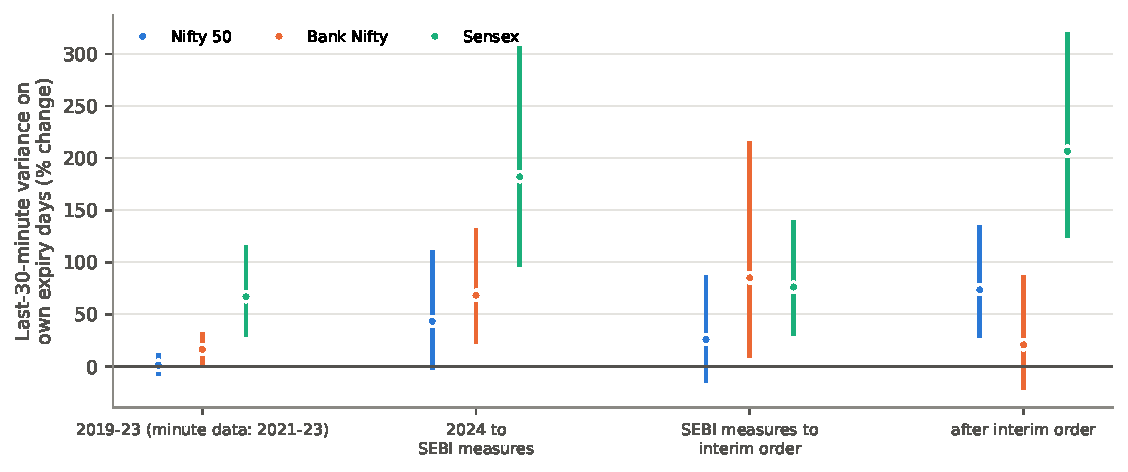
\includegraphics[width=0.95\textwidth]{fig6_periods.pdf}
\caption{\textbf{The settlement-window effect over time.} Own-expiry effect on 15:00--15:30 realized variance, by index and period, compared with the other indices on the same weekday and week; 95\% intervals.}
\label{fig:periods}
\end{figure}


% ===========================================================================
\section{Total volatility and forecasting}\label{sec:forecast}
\paragraph{Does expiry create volatility or move it?}
\begin{itemize}
\item Weeks in which an index has weekly options show 5.5\% higher total variance in a simple two-way fixed-effects comparison ($p=0.002$).
\item With index-specific trends the difference is $-1.8\%$ ($p=0.30$), and individual launches and removals give estimates of both signs.
\item So there is no reliable evidence that weekly options raise an index's total volatility.
\end{itemize}

\paragraph{Forecasting.}
\begin{itemize}
\item The earlier paper on Nifty volatility forecasting found that a HAR model \citep{corsi2009}, fitted with the QLIKE-matching loss \citep{patton2011}, is hard to beat.
\item Here, adding the next day's expiry indicators, which are known in advance, makes walk-forward forecasts from 2018 slightly \emph{worse}: QLIKE rises by 1.0--1.8\% for the three large indices, with Diebold--Mariano \citep{diebold1995} $p$-values from 0.01 to 0.06 (Table~\ref{tab:forecast}).
\item Daily volatility models therefore gain nothing from the calendar. This is consistent with the effect being concentrated in a half hour that daily measures barely register.
\end{itemize}

\begin{table}[t]
\centering
\caption{\textbf{Does the calendar help forecasting?} Walk-forward forecasts of next-day close-to-close variance, January 2018 -- July 2026, expanding window re-fitted every 22 days. HAR inputs: log variance over the last day, week and month and the calendar days to the next session; ``+ calendar'' adds the next day's own weekly, own monthly and other-large-index expiry indicators. QLIKE: lower is better. DM: Diebold--Mariano test with Newey--West errors.}
\label{tab:forecast}
\small
\fittable{forecast}
\end{table}


% ===========================================================================
\section{Discussion and limitations}
\begin{itemize}
\item \textbf{Shared stocks:} the indices share stocks, so ``own'' and ``other'' expiry effects are not cleanly separable. The within-index estimates capture total effects. The cross-index estimates capture the part specific to the expiring index.
\item \textbf{Short windows after recent changes:} the minute data begin in 2021, and the most recent calendar changes have only six to ten months of data after them.
\item \textbf{Volume and prices:} realized variance from index levels does not distinguish price pressure that reverses from information. The reversal and pinning tests only partly address this.
\item \textbf{Daily data quality:} early daily opening prices for Bank Nifty and Midcap~50 look stale. Results starting in 2017 are similar.
\item \textbf{The calendar:} it is rule-based. It is verified against exchange files for Nifty, Bank Nifty and Sensex, but not for the three small products, which enter only as controls.
\end{itemize}

% ===========================================================================
\section{Conclusion}
\begin{itemize}
\item India's frequent changes to its options expiry calendar give a clean test of whether expiry destabilises markets.
\item The answer is narrower than the debate suggests. Expiry days are at most slightly more volatile overall, but the half hour that sets the settlement price is much more volatile, and this volatility moves with the expiry calendar.
\item For market stability, policies aimed at how settlement prices are formed, such as closing auctions, settlement averaging windows or position monitoring in the final minutes, target the volatility that the data show. Whether India's new closing auction achieves this is an open question.
\end{itemize}

\section*{Data and code availability}
\begin{itemize}
\item All code is available at \url{https://github.com/vicky123411/india-options-expiry-effects}. It includes the expiry calendar, the holiday list, the tests and notebooks that reproduce every table and figure.
\item Price data are downloaded from their sources on first run and are not redistributed.
\end{itemize}

\section*{Declarations}
% TODO (author): adapt to the target journal's policy before submission.
\textbf{Funding:} none. \textbf{Competing interests:} none. \textbf{Use of AI tools:} AI assistants (Claude, Anthropic) were used to write analysis code and to draft and edit the text; the author is responsible for the content.

\bibliographystyle{plainnat}
\bibliography{references}

% ===========================================================================
\clearpage
\appendix
\section{Additional results}
\begin{table}[h]
\centering
\caption{\textbf{Alternative whole-session outcomes} (pooled, equation~\eqref{eq:main}). The overnight gap is the squared return from the previous close to the open of the expiry day.}
\label{tab:alt}
\scriptsize
\setlength{\tabcolsep}{4pt}
\fittable{alt_outcomes}
\end{table}

\begin{table}[h]
\centering
\caption{\textbf{The closing auction: an early look.} Log Parkinson variance of the last hourly bar (15:15--15:30), October 2023 -- September 2026. ``After'' = from 3 August 2026 (two months). Pooled: index$\times$weekday and index$\times$week effects; per index: weekday and week effects. Low power: few expiry days after the change.}
\label{tab:cas}
\scriptsize
\fittable{closing_auction}
\end{table}

\begin{figure}[h]
\centering
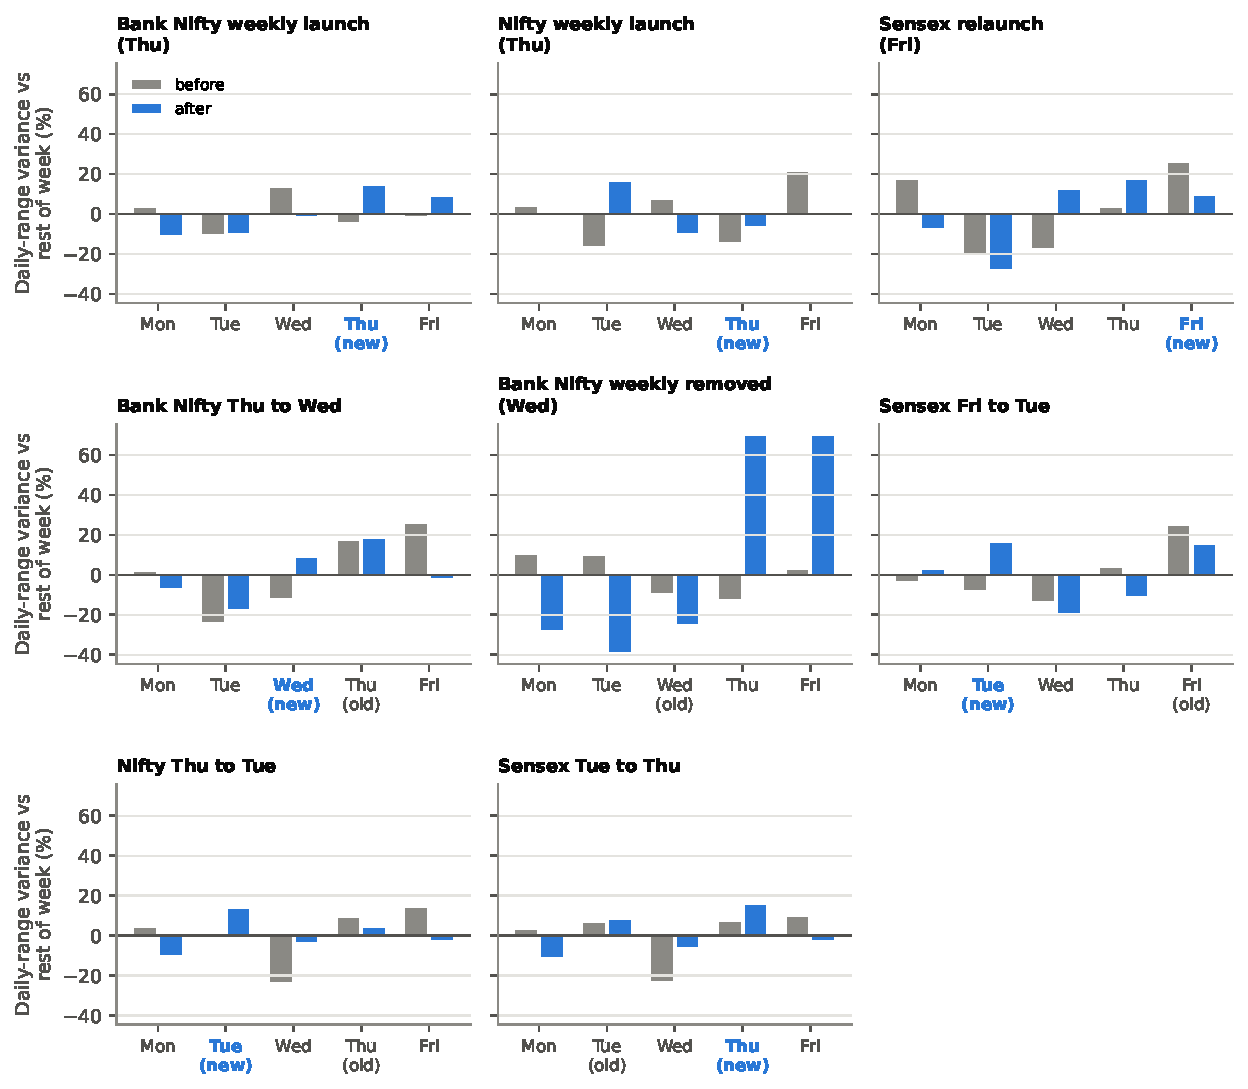
\includegraphics[width=\textwidth]{figA1_moving_day.pdf}
\caption{\textbf{Whole-session volatility around the eight major calendar changes} (daily data, log Garman--Klass variance relative to the rest of the week). Unlike the closing window (Figure~\ref{fig:moving}), the weekday profile does not consistently follow the expiry day.}
\label{fig:movingday}
\end{figure}

\begin{figure}[h]
\centering
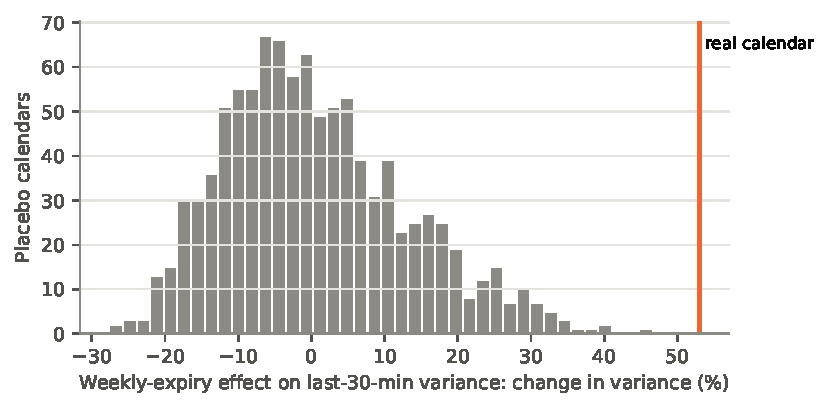
\includegraphics[width=0.7\textwidth]{figA2_placebo_last30.pdf}
\caption{\textbf{Placebo calendars.} Estimated weekly-expiry effect on 15:00--15:30 variance under 1,000 placebo calendars that keep the dates of every rule change but draw the weekdays at random; the vertical line is the estimate with the real calendar.}
\label{fig:placebo}
\end{figure}


\end{document}
